\let\negmedspace\undefined
\let\negthickspace\undefined
\documentclass[journal]{IEEEtran}
\usepackage[a5paper, margin=10mm, onecolumn]{geometry}
%\usepackage{lmodern} % Ensure lmodern is loaded for pdflatex
\usepackage{tfrupee} % Include tfrupee package

\setlength{\headheight}{1cm} % Set the height of the header box
\setlength{\headsep}{0mm}     % Set the distance between the header box and the top of the text

\usepackage{gvv-book}
\usepackage{gvv}
\usepackage{cite}
\usepackage{amsmath,amssymb,amsfonts,amsthm}
\usepackage{algorithmic}
\usepackage{graphicx}
\usepackage{textcomp}
\usepackage{xcolor}
\usepackage{txfonts}
\usepackage{listings}
\usepackage{enumitem}
\usepackage{mathtools}
\usepackage{gensymb}
\usepackage{comment}
\usepackage[breaklinks=true]{hyperref}
\usepackage{tkz-euclide} 
\usepackage{listings}
\def\inputGnumericTable{}                                 
\usepackage[latin1]{inputenc}                                
\usepackage{color}                                            
\usepackage{array}                                            
\usepackage{longtable}                                       
\usepackage{calc}                                             
\usepackage{multirow}                                         
\usepackage{hhline}                                           
\usepackage{ifthen}                                           
\usepackage{lscape}
\begin{document}

\bibliographystyle{IEEEtran}


\title{4.12.17}
\author{AI25BTECH11012 - GARIGE UNNATHI}
% \maketitle
% \newpage
% \bigskip
{\let\newpage\relax\maketitle}


\renewcommand{\thefigure}{\theenumi}
\renewcommand{\thetable}{\theenumi}
\setlength{\intextsep}{10pt} % Space between text and floats


\numberwithin{equation}{enumi}
\numberwithin{figure}{enumi}

\vspace{-1cm}

\textbf{Question}:\\
$\vec{P1}$,$\vec{P2}$ are points on either of the two lines y - $\sqrt{3}$$\lvert x \rvert$ = 2 at a distance of 5 units from their point of intersection. Find the coordinates of the foot of the perpendiculars drawn from $\vec{P1}$,$\vec{P2}$ on the bisector of the angle between the given lines.\\

\textbf{Solution:}\\

The equation of the lines is :
\begin{align}
  y - \sqrt{3}x = \myvec{-\sqrt{3} & 1}\myvec{x\\y} = 2\\
   y + \sqrt{3}x = \myvec{\sqrt{3} & 1}\myvec{x\\y} = 2 
\end{align}
Combining both the equations 0.1 and 0.2 ,we get :
\begin{align}
   \myvec{-\sqrt{3} & 1\\
           \sqrt{3} & 1 }\myvec{x\\y} = \myvec{2\\2}
\end{align}
Solving by row reduction we get :

\begin{align}
\vec{Q} = \myvec{0\\2}
\end{align}

The equation for the point $\vec{P_1}$ are:
\begin{align}
\myvec{\sqrt{3} & 1}\vec{P_1} = 2\\
\lVert \vec{P_1} -  \vec{Q} \rVert = 5
\end{align}

The equation for the point $\vec{P_2}$ are:

\begin{align}
\myvec{-\sqrt{3} & 1}\vec{P_2} = 2\\
\lVert \vec{P_2} -  \vec{Q} \rVert = 5
\end{align}

Solving the equations we get :
\begin{align}
   \vec{P_1} = \myvec{\frac{5}{2} \\ 2+\frac{5\sqrt{3}}{2}} \\
    \vec{P_2} = \myvec{-\frac{5}{2} \\ 2-\frac{5\sqrt{3}}{2}}
\end{align}

The equation of the angle bisector is given by \\
Let us take a point $\vec{P}$ on the angle bisector , substitution it in the line equtions and equating the angles we get the equation :
\begin{align}
  \frac{\lvert n_1\vec{P} - 2 \rvert}{\lVert n_1\rVert}  =  \frac{\lvert n_2\vec{P} - 2 \rvert}{\lVert n_1\rVert} \\
  \frac{n_1\vec{P} - 2}{\lVert n_1\rVert} \pm \frac{ n_2\vec{P} - 2}{\lVert n_1\rVert} = 0
\end{align}
solving the above equation we get locus of $\vec{P}$ as two lines which are the angle bisectors :

\begin{align}
    \myvec{1\\0}^{T}\vec{x} = 0\\
     \myvec{0\\1}^{T}\vec{x} = 2
\end{align}

Let Q be the foot of the perpendicular from P to the line
\begin{align}
    \vec{n}^{T}\vec{x} = c
\end{align}
Then :
\begin{align}
    \myvec{\vec{m}&\vec{n}}^{T}\vec{Q} = \myvec{\vec{m}^{T}\vec{P}\\c}
\end{align}

solving this equation for the line $\myvec{1\\0}^{T}\vec{x} = 0$ ,we get :
\begin{align}
    \myvec{0\\2+\frac{5\sqrt{3}}{2}} \quad and \quad \myvec{0\\2-\frac{5\sqrt{3}}{2}}
\end{align}
and solving it for the line $\myvec{0\\1}^{T}\vec{x} = 2$, we get :
\begin{align}
    \myvec{\frac{5}{2} \\ 2} \quad and \quad \myvec{-\frac{5}{2} \\ 2}
\end{align}



\begin{figure}[h!]
   \centering
   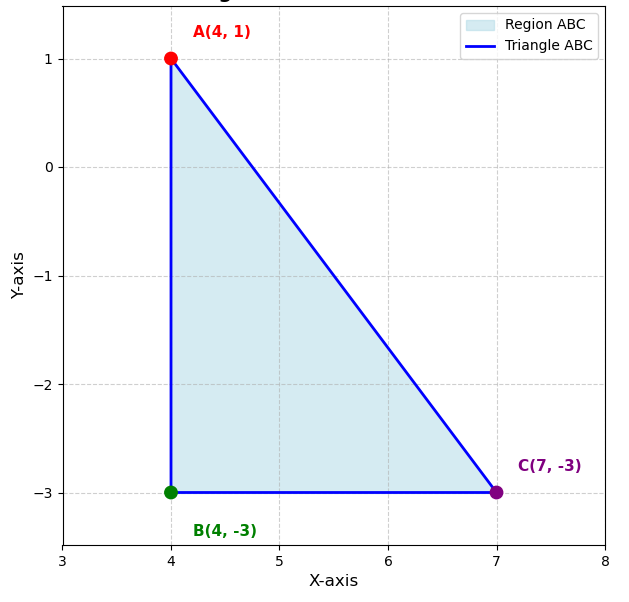
\includegraphics[width=0.7\linewidth]{/Users/unnathi/Documents/ee1030-2025/ai25btech11012/matgeo/4.12.17/figs/fig.png}
   \caption{}
   \label{stemplot}
\end{figure}


\end{document}

 
